\subsection{Boundary conditions for Lid-Driven Cavity problem}
\label{subsec:boundary_conditions_for_lid_driven}

So far, we have presented all the tools and concepts required to solve a generic fluid flow problem (except for the algorithm itself) that respect the hypothesis and conditions stated at the beginning of Section \ref{sec:derivation_of_discretized_governing_equations}.

In this section we will present the boundary conditions that will be used to solve the Lid-Driven Cavity problem and their implementation inside the \acrshort{scgs} method.



\subsubsection{Ghosts cells}

Consider that our domain has already been discretized (subdivided) into $N_x \times N_y$ cells.

If we think of the scheme for both the convection and diffusion presented before, we can see that at the boundary of our domain, the coefficients $A_p\phi$ \ref{tab:Ap_coefficients} involve cells that are outside the domain.
For this reason, we need to add a layer of cells outside the physical domain, called ghost cells, to calculate the coefficients at the boundary.

The number of ghost cells required depends on the order of the scheme used to calculate the coefficients. For a second-order scheme, we need at least one ghost cell, and for a fourth-order scheme, we need at least two ghost cells.

Here, and also in the implementation of the \acrshort{scgs} method in the code, we will consider the possibility to adopt a mixed strategy scheme and use:

\begin{itemize}
    \item Away from boundaries: higher-order schemes
    \item Near boundaries: \acrshort{uds} scheme for convection and 2nd-order scheme for diffusion
\end{itemize}

By doing so, we ensure that at the boundaries both the schemes will be applicable with just a single layer of ghost cells.

\begin{figure}[H]
    \centering
    \def\nCV{5}
    \def\dX{1.5cm}
    \def\dY{1.5cm}

    \begin{tikzpicture}

        \foreach \n in {0,1,...,\nCV}
            {
                \draw (0, \n*\dY) -- (\nCV*\dX, \n*\dY);
                \draw (\n*\dX, 0) -- (\n*\dX, \nCV*\dY);
            }

        % \foreach \n in {0,1,...,\the\numexpr\nCV-1\relax}
        %     {
        %         \draw[dashed] (-\dX/2, \n*\dY + \dY/2) -- (\nCV*\dX+\dX/2, \n*\dY + \dY/2);
        %         \draw[dashed] (\n*\dX + \dX/2, -\dY/2) -- (\n*\dX + \dX/2, \nCV*\dY+\dY/2);
        %     }

        \foreach \y in {0,1,...,\the\numexpr\nCV-1\relax}
            {
                \foreach \x in {0,1,...,\the\numexpr\nCV-1\relax}
                    {
                        \node[font=\small] at (\x*\dX+\dX/6, \y*\dY+\dY/10) {$_{\the\numexpr\x+0\relax,\the\numexpr\y+0\relax}$};
                    }
            }

        \draw[line width=0.5mm] (\dX, \dY) -- (\dX, \nCV*\dY-\dY) -- (\nCV*\dX-\dX, \nCV*\dY-\dY) -- (\nCV*\dX-\dX, \dY) -- cycle;

        % \fill[red, opacity=0.1] (0, 0) rectangle (\nCV*\dX, \nCV*\dY);
        \fill[yellow, opacity=0.3] (\dX, \dY) rectangle (\nCV*\dX-\dX, \nCV*\dY-\dY);

    \end{tikzpicture}
    \caption{Physical domain and ghost cells}
    \label{fig:ghost_cells}
\end{figure}

In Figure \ref{fig:ghost_cells}, the yellow area represents the physical domain, while the frame surrounding it represents the ghost cells.

As we can see, the indexes of the cells stick to the physical domain, while the ghost cells may have negative indexes.

In the case above, we can declare some of the problem that will be recalled during the following sections:

\begin{itemize}
    \item Physical domain: $N_x \times N_y$ grid. In the example above, $N_x = N_y = 3$
    \item Physical domain indexes: from $(1,1)$ to $(3,3)$. In general, from $(1,1)$ to $(N_x,N_y)$.
    \item Ghost cells layer: may have different sizes along the $x$ and $y$ directions. In the example above, the ghost cells layer has a size of $N_g = 1$ cell in both directions. We will stick with this size for the rest of the document.
    \item Ghost cells indexes: may have negative indexes. In the example above, the ghost cells have indexes from $(0,0)$ to $(4,4)$, that is equivalent to $(1-N_g,1-N_g)$ to $(N_x+2*N_g-1,N_y+2*N_g-1)$.
\end{itemize}

We can now proceed to identify the boundary conditions for the Lid-Driven Cavity problem.



\subsubsection{No-slip condition}

As boundary conditions for the Lid-Driven Cavity problem (and for most of the fluid flow problems), we have the no-slip condition, which gives us the constraint for two direction of the velocity field:

\begin{itemize}
    \item Component normal to the wall: given a condition of impenetrability, the velocity component normal to the wall must be zero (no-penetration)
    \item Component tangential to the wall: given a condition of no-slip, the velocity component tangential to the wall must equal to the wall velocity
\end{itemize}

As an example, we can consider the cell in position $(1, N_y)$, which is the top-left corner of the physical domain (Figure \ref{fig:ghost_cells} for reference).

\begin{figure}[H]
    \centering
    \def\nCV{2}
    \def\dX{3cm}
    \def\dY{3cm}

    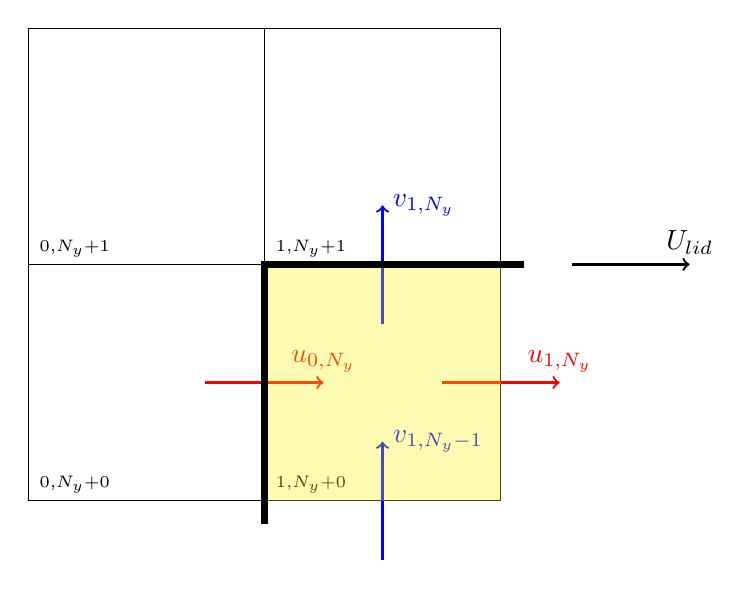
\begin{tikzpicture}

        \foreach \n in {0,1,...,\nCV}
            {
                \draw (0, \n*\dY) -- (\nCV*\dX, \n*\dY);
                \draw (\n*\dX, 0) -- (\n*\dX, \nCV*\dY);
            }

        \foreach \y in {0,1,...,\the\numexpr\nCV-1\relax}
            {
                \foreach \x in {0,1,...,\the\numexpr\nCV-1\relax}
                    {
                        \node[font=\small] at (\x*\dX+\dX/5, \y*\dY+\dY/15) {$_{\x, N_y+\y}$};
                    }
            }

        \draw[thick, blue, ->] (3/2*\dX, 1/2*\dY)++(0,  \dY/4) -- ++(0, \dY/2) node[pos=1, right] {$v_{1,N_y}$};
        \draw[thick, blue, ->] (3/2*\dX, 1/2*\dY)++(0, -\dY/2-\dY/4) -- ++(0, \dY/2) node[pos=1, right] {$v_{1,N_y-1}$};
        \draw[thick, red, ->] (3/2*\dX, 1/2*\dY)++(\dX/4, 0) -- ++(\dX/2, 0) node[pos=1, above] {$u_{1,N_y}$};
        \draw[thick, red, ->] (3/2*\dX, 1/2*\dY)++(-\dX/2-\dX/4, 0) -- ++(\dX/2, 0) node[pos=1, above] {$u_{0,N_y}$};

        \fill[yellow, opacity=0.3] (\dX, 0) rectangle (2*\dX, \dY);

        \draw[line width=1mm] (\dX, -\dY/10) -- (\dX, \dY) -- (2*\dX+\dX/10, \dY);
        \draw[thick, ->] (2*\dX +\dX/10, \dY) ++(\dX/5, 0) -- ++(\dX/2, 0) node[pos=1, above] {$U_{lid}$};

    \end{tikzpicture}
    \caption{Boundary conditions for the cell $(1, N_y)$}
    \label{fig:boundary_conditions_1Ny}
\end{figure}

In this case, we must accomplish the following conditions:

\begin{itemize}
    \item $u_{0, N_y} = 0$ (no-penetration)
    \item $v_{1, N_y} = 0$ (no-penetration)
    \item $u_{1, N_y} = U_{lid}$ (no-slip)
\end{itemize}

Intuitively, we can understand that similar conditions must be applied to the other walls of the domain given the correction of the indexes and the direction of the velocity field.

In general, we can state that the boundary conditions for the Lid-Driven Cavity problem are:

\begin{itemize}
    \item Bottom wall: $v_{i,0} = 0$ (no-penetration) + $u_{i,1} = 0$ (no-slip)
    \item Left wall: $u_{0,j} = 0$ (no-penetration) + $v_{1,j} = 0$ (no-slip)
    \item Top wall: $v_{i,N_y} = 0$ (no-penetration) + $u_{i,N_y} = U_{lid}$ (no-slip)
    \item Right wall: $u_{N_x,j} = 0$ (no-penetration) + $v_{N_x,j} = 0$ (no-slip)
\end{itemize}

We can now proceed to see how these conditions are accounted for in the \acrshort{scgs} method.



\subsubsection{Boundary conditions inside \acrshort{scgs} method}

By adopting the \acrshort{scgs} method, we can impose the boundary conditions in the following way:

\begin{itemize}
    \item No-penetration condition: impose specific coefficients in the Vanka matrix to be zero
    \item No-slip condition: impose specific velocity values in the ghost cells
\end{itemize}

Moreover, as we are going to see, the no-penetration condition imply the velocity to be null and can be imposed to the system before solving the linear system of equations.
Instead, given the mathematical formulation of the no-slip condition, we can impose the velocity values in the ghost cells only after solving the linear system of equations (and will affect the next iteration).

\paragraph{No-penetration condition}

The no-penetration condition imply the normal velocity component at the boundary to be null.
This means that if we start from an initial guess of the velocity field equal to zero everywhere, we must ensure that correction of the velocity field at the boundary is null for each iteration.

Taken for example the cell $(1, N_y)$ as in Figure \ref{fig:boundary_conditions_1Ny}, we know that we must impose $u_{0, N_y} = 0$ \& $v_{1, N_y} = 0$, which means that the correction of the velocity field at the boundary must be null as well $u_{0, N_y}' = 0$ \& $v_{1, N_y}' = 0$.

By recalling the formulation for both the continuity and momentum equations, we can see that multiple terms must be canceled out (known null solution).

For the \textbf{continuity equation} written at the cell $(1, N_y)$, we have:

\begin{equation}
    -u_{0, N_y}' \Delta y + u_{1, N_y}' \Delta y - v_{1, N_y-1}' \Delta x + v_{1, N_y}' \Delta x = R_{1, N_y}^c
\end{equation}

By imposing $[A^\phi]_{5,1} = \Delta y = 0$, we can cancel out the first term, and by imposing $[A^\phi]_{5, 4} = \Delta x = 0$, we can cancel out the third term.

In this way, even if we are not imposing the no-penetration condition directly, we are imposing an equivalent condition that will lead to the same result.

More in general, given the physical domain of size $N_x \times N_y$, we can impose the no-penetration condition for the continuity equation by setting:

\begin{align}
    @i=1, u_{i-1, j}' = 0 \rightarrow [A^\phi]_{5,1} & = - \Delta y = 0 \quad \forall j = 1,2,...,N_y \\
    @i=N_x, u_{i, j}' = 0 \rightarrow [A^\phi]_{5,2} & = \Delta y = 0 \quad \forall j = 1,2,...,N_y   \\
    @j=1, v_{i, j-1}' = 0 \rightarrow [A^\phi]_{5,3} & = - \Delta x = 0 \quad \forall i = 1,2,...,N_x \\
    @j=N_y, v_{i, j}' = 0 \rightarrow [A^\phi]_{5,4} & = \Delta x = 0 \quad \forall i = 1,2,...,N_x
\end{align}

For the \textbf{momentum equations}, written at the cell $(1, N_y)$ for the two components that are controlled by the no-penetration condition, we have:

\begin{align}
    (A_P^u)_{0,N_y} u_{0,N_y}' + p_{0,N_y}' \Delta y & = R^u_{0,N_y} \\
    (A_P^v)_{1,N_y} v_{1,N_y}' - p_{1,N_y}' \Delta x & = R^v_{1,N_y}
\end{align}

By imposing $[A^\phi]_{1,5} = \Delta y = 0$ and $[R^\phi]_{1} = 0$, we can cancel out the first equation, and by imposing $[A^\phi]_{4,5} = - \Delta x = 0$ and $[R^\phi]_{4} = 0$, we can cancel out the second equation.

More in general, given the physical domain of size $N_x \times N_y$, we can impose the no-penetration condition for the momentum equations by setting:

\begin{align}
    @i=1, u_{i-1, j}' = 0 \rightarrow [A^\phi]_{1,5} & = \Delta y = 0 \quad \forall j = 1,2,...,N_y   \\
    @i=N_x, u_{i, j}' = 0 \rightarrow [A^\phi]_{2,5} & = - \Delta y = 0 \quad \forall j = 1,2,...,N_y \\
    @j=1, v_{i, j-1}' = 0 \rightarrow [A^\phi]_{3,5} & = \Delta x = 0 \quad \forall i = 1,2,...,N_x   \\
    @j=N_y, v_{i, j}' = 0 \rightarrow [A^\phi]_{4,5} & = - \Delta x = 0 \quad \forall i = 1,2,...,N_x
\end{align}

\paragraph{No-slip condition}

The idea behind the no-slip condition for the tangential velocity component is to impose the velocity field in the ghost cells so that the interpolation with the velocity field in the physical domain gives the correct value at the boundary.

As an example, we can consider the cell $(1, N_y)$ as in Figure \ref{fig:boundary_conditions_1Ny}.

We know that we must impose $u_{1, N_y} = U_{lid}$.
Given that the condition can't be imposed directly to the correction term as for the no-penetration condition, here we have to solve the system and then impose the condition over the ghost cells velocity based on the current solution of the velocity field.

In particular, we can think of the wall velocity as the average of the velocity in the ghost cell and the velocity in the physical domain.
This implies to impose the following condition for the cell $(1, N_y)$:

\begin{equation}
    U_{lid} = \frac{1}{2} (u_{1, N_y} + u_{1, N_y+1}) \rightarrow u_{1, N_y+1} = 2 U_{lid} - u_{1, N_y}
\end{equation}

More in general, given the physical domain of size $N_x \times N_y$, we can impose the no-slip condition for the velocity field by setting:

\begin{align}
    @i=1, v_{0, j}       & = - v_{1, j} \quad \forall j = 1,2,...,N_y             \\
    @i=N_x, v_{N_x+1, j} & = - v_{N_x, j} \quad \forall j = 1,2,...,N_y           \\
    @j=1, u_{i, 0}       & = - u_{i, 1} \quad \forall i = 1,2,...,N_x             \\
    @j=N_y, u_{i, N_y+1} & = 2 U_{lid} - u_{i, N_y} \quad \forall i = 1,2,...,N_x
\end{align}